% bs-Script
% Kapitel 2
%
Für die Behandlung der Anforderungen in Mehrprogrammbetriebssystemen 
sind primitive Ad-hoc-Lösungen nicht mehr möglich. Das Verständnis des 
Gesamtsystems ist nicht mehr durch die Beschreibung des Verhaltens der 
CPU zu jedem Zeitpunkt möglich, da das Verhalten der CPU 
in Mehrbenutzersystemen im Mehrprogrammbetrieb stark
von nicht vorhersagbaren externen Ereignissen (Unterbrechungen) abhängig 
ist.
Das Betriebssystem wird als Ansammlung von funktionellen Einheiten 
betrachtet, die zunächst unabhängig voneinander arbeiten aber über
 wohldefinierte Schnittstellen miteinander kommunizieren müssen.
Diese funktionellen Einheiten bezeichnet man als Prozesse.
\section{Prozeßbegriff}

\paragraph{Typische Merkmale von Prozessen:} \ \\
\begin{itemize}
\item   brauchen Prozessor
\item   enthalten jeweils ein sequentielles Programm
\item   können grundsätzlich parallel ablaufen
\end{itemize}

Zur Abgrenzung zum Begriff \emph{Benutzerauftrag} (\emph{Job}): Zur 
Abarbeitung eines Benutzerauftrags sind in der Regel mehrere Prozesse 
notwendig.
\paragraph{Formen der Parallelität}
\begin{itemize}
\item   mehrere Prozesse laufen auf unterschiedlichen Prozessoren ab \\
	(tatsächlich parallel)
\item   ein Prozessor wird "`scheibchenweise"' den Prozessen zugeordnet, so daß
	diese "`überlappt"' ablaufen \\
	(quasi-parallel)
\end{itemize}
Die im Zusammenhang mit der Parallelität von Prozessen auftretenden 
Probleme sind davon aber unabhängig.
\section{Synchronisation konkurrierender und kooperierender Prozesse}
\subsection{Problem des wechselseitigen Ausschlusses}
Das Problem des wechselseitigen Ausschlusses ({\em mutual exclusion}) wurde
erstmals 1965 von \textsc{Edsger W. Dijkstra} formuliert.
\paragraph{Beispiel 1:}
Zwei zyklische Prozesse $p_1$ und $p_2$ benutzen von Zeit zu Zeit
ein Magnetband. Es steht nur ein Gerät zur Verfügung, das nicht von 
mehr als einem Prozeß gleichzeitig benutzt werden kann.
\subparagraph{1. Lösungsversuch:}
man definiert eine boolesche Variable \texttt{frei} \\

\begin{minipage}{6cm}
\hspace*{1cm} \\
$p_1$:
\ttfamily
\begin{tabbing}
\hspace*{1cm}\=\hspace{5mm}\=\hspace{5mm}\= \kill
001\>   wiederhole \\
002\>   \>      wiederhole bis frei; \\
003\>   \>      frei := false; \\
004\>   \>      benutze(magnetband) \\
005\>   \>      frei := true; \\
$\vdots$\>\>    $\vdots$ \\
FFF\>   ständig \\
\end{tabbing}
\end{minipage}
\begin{minipage}{6cm}
\hspace*{1cm} \\
$p_2$: 
\ttfamily
\begin{tabbing}
\hspace*{1cm}\=\hspace{5mm}\=\hspace{5mm}\= \kill
001\>   wiederhole \\
002\>   \>      wiederhole bis frei; \\
003\>   \>      frei := false; \\
004\>   \>      benutze(magnetband) \\
005\>   \>      frei := true; \\
$\vdots$\>\>    $\vdots$ \\
FFF\>   ständig \\
\end{tabbing}
\end{minipage}

\subparagraph{Problem:} Wenn $p_1$ und $p_2$  parallel ablaufen, können sie 
auch gleichzeitig das Magnetband als frei erkennen. Das gleiche Problem 
kann auch bei quasi-parallel ablaufenden Prozessen auftreten, da jeder Prozeß
zwischen \texttt{002} und \texttt{003} unterbrochen werden kann.

Weiterer Nachteil dieser "`Lösung"': Durch die Warteschleife wird 
Prozessorzeit beansprucht ({\em busy waiting}).

\subparagraph{2. Lösungsversuch}
man definiert eine boolesche Variable \texttt{p1anderReihe} \\

\begin{minipage}{6cm}
\hspace*{1cm} \\
$p_1$:
\ttfamily
\begin{tabbing}
\hspace*{1cm}\=\hspace{5mm}\=\hspace{5mm}\= \kill
001\>   wiederhole \\
002\>   \>      wiederhole bis p1anderReihe; \\
003\>   \>      benutze(magnetband) \\
004\>   \>      p1anderReihe := false; \\
$\vdots$\>\>    $\vdots$ \\
FFF\>   ständig \\
\end{tabbing}
\end{minipage}

\begin{minipage}{6cm}
\hspace*{1cm} \\
$p_2$: 
\ttfamily
\begin{tabbing}
\hspace*{1cm}\=\hspace{5mm}\=\hspace{5mm}\= \kill
001\>   wiederhole \\
002\>   \>      wiederhole bis nicht p1anderReihe; \\
003\>   \>      benutze(magnetband) \\
004\>   \>      p1anderReihe := true; \\
$\vdots$\>\>    $\vdots$ \\
FFF\>   ständig \\
\end{tabbing}
\end{minipage}

Ein wechselseitiger Ausschluß ist zwar gewährleistet, allerdings müssen die
Prozesse das Magnetband abwechselnd benutzen. Beide Prozesse müssen außerdem
"`am Leben"' bleiben. {\em Busy waiting} tritt auch hier auf.

\subparagraph{3. Lösungsversuch}
Definition zweier boolesche Variablen \texttt{p1istdran} und \texttt{p2istdran}

Initialisierung:
\ttfamily
\begin{tabbing}
\hspace*{5mm}\=\kill
\>	p1istdran := false\\
\>	p2istdran := false
\end{tabbing}
\rmfamily
\begin{minipage}[t]{6cm}
p1:
\ttfamily
\begin{tabbing}
\hspace*{5mm}\=\kill
wiederhole\\
\>	p1istdran := true\\
\>	wiederhole bis nicht p2istdran\\
\>	benutze(magnetband)\\
\>	p1istdran := false\\
\>	$\vdots$\\
ständig
\end{tabbing}
\end{minipage}
\begin{minipage}[t]{6cm}
p2:
\ttfamily
\begin{tabbing}
\hspace*{5mm}\=\kill
wiederhole\\
\>	p2istdran := true\\
\>	wiederhole bis nicht p1istdran\\
\>	benutze(magnetband)\\
\>	p2istdran := false\\
\>	$\vdots$\\
ständig
\end{tabbing}
\end{minipage}\\

Wechselseitiger Ausschluß ist zwar garantiert, es besteht aber die Gefahr der 
Verklemmung ({\em deadlock}).

Anforderungen an eine Lösung für das Problem des wechselseitigen Ausschlusses:
\begin{enumerate}
\item	Das Betriebsmittel wird nach endlicher Zeit zugewiesen.
\item	Ein Prozeß gibt das Betriebsmittel nach endlicher Zeit wieder frei.
\item	Ein Prozeß, der wartet, soll keine Rechenzeit verbrauchen.
\item	Eine Problemlösung soll von den Prozessen in eine gemeinsame Umgebung
	verlagert werden.
\end{enumerate}

Das grundsätzliche Problem resultiert aus der "`unkontrollierten"' Benutzung gemeinsamer 
Daten.
 
Weitere Beispiele für das Auftreten des Problems des wechselseitigen 
Ausschlusses:
\begin{enumerate}
	\item  Veränderung von Datensätzen in einer von mehreren Prozessen 
	gemeinsam benutzten Datei

	\item  gemeinsame Benutzung von Unterprogrammen mit lokalen Variablen 
	für Zwischenergebnisse
\end{enumerate}

\paragraph{Definition:} Programmabschnitte, in denen sich zu einem 
Zeitpunkt nur jeweils ein Prozeß befinden darf, heißen \emph{kritische 
Abschnitte} (\emph{critical sections}).

\paragraph{Lösung:
\texttt{P}- und \texttt{V}-Operationen nach \textsc{Edsger W. Dijkstra}} 
\ \\
\texttt{P} und \texttt{V} sind zwei Operationen auf einer gemeinsamen Variablen,
genannt \emph{Semaphorvariable}.
Jedem kritischen Abschnitt wird eine Semaphore zugeordnet.

\paragraph{Definition von \texttt{P} und \texttt{V}:}
\begin{verbatim}
P(s):
   wenn s=1
   dann s:=0
   sonst blockiere den aufrufenden Prozess
         und schalte auf anderen Prozess um
	
V(s):
   wenn ein Prozess auf s wartet
   dann loese den Prozeß aus Wartezustand
   sonst s:=1
\end{verbatim}

Beispiel für die Sicherung eines kritischen Abschnitts (Benutzung eines 
Magnetbandgeräts) durch eine Semaphore \texttt{s}:
\ttfamily
\begin{tabbing}
\hspace*{5mm}\=\kill
\>	P(s)\\
\>	benutze(magnetband)\\
\>	V(s)
\end{tabbing}
\rmfamily

\texttt{P}- und \texttt{V}-Operationen sind selbst kritische Abschnitte
und müssen atomar sein (dürfen nicht selbst unterbrochen werden).
Es handelt sich aber um kurze kritische Abschnitte, die im Systemkern 
realisiert werden, wo wechselseitiger Ausschluß einfach zu 
implementieren ist.
Sie werden häufig mithilfe eines Spezialbefehls des Prozessors realisiert, wobei 
ein aktives Warten in Kauf genommen wird. Dazu wird eine
Sperrvariable \texttt{pv} mit folgender Bedeutung eingeführt:

\bigskip
\begin{tabular}{lcl}
	\texttt{pv=1} & : & \texttt{P}- und \texttt{V}-Operationen können ausgeführt werden \\
	\texttt{pv=0} & : & \texttt{P}- und \texttt{V}-Operationen können nicht ausgeführt werden
\end{tabular}
\bigskip

Der Spezialbefehl \texttt{teste\_und\_setze(pv)} ist eine
unteilbare Operation, die folgendermaßen arbeitet:

\begin{verbatim}
   wiederhole solange pv = 0; (* tue nichts, busy waiting *)\\
   pv := 0
\end{verbatim}

Mithilfe dieses Befehls werden nun zwei modifizierte Operationen
 \texttt{P'} und \texttt{V'} eingeführt, die dann zur Sicherung eines
 kritischen Abschnitts eingesetzt werden können.

\bigskip
\begin{minipage}[t]{6cm}
\ttfamily
\begin{tabbing}
\hspace*{5mm}\=\kill
P'(s)\\
\>	teste\_und\_setze(pv)\\
\>	P(s)\\
\>	pv:=1
\end{tabbing}
\end{minipage}
\hspace{1cm}
\begin{minipage}[t]{6cm}
\ttfamily
\begin{tabbing}
\hspace*{5mm}\=\kill
V'(s)\\
\>	teste\_und\_setze(pv)\\
\>	V(s)\\
\>	pv:=1
\end{tabbing}
\end{minipage}

\bigskip
Bisher wurden nur um gemeinsame Betriebsmittel konkurrierende Prozesse 
betrachtet, die sonst nichts miteinander zu tun hatten.

\subsection{Synchronisation kooperierender Prozesse}
Kooperation zwischen Prozessen kann z.B. heißen, daß Nachrichten 
zwischen einem Erzeuger und einem Verbraucher ausgetauscht werden
({\em producer-consumer-pro"-blem}).

Nachrichtenaustausch soll gepuffert erfolgen, um Erzeuger und Verbraucher
bezüglich ihrer Arbeitsgeschwindigkeit zu entkoppeln.
Ringpuffer fester Größe kann nur eine feste Anzahl von Nachrichten 
speichern. Abbildung \ref{Ringpuffer} zeigt einen teilweise gefüllten 
Ringpuffer mit zwei Zeigern, \texttt{c} für den Verbraucher und 
\texttt{p} für den Erzeuger. Beide Prozesse bearbeiten den Puffer im 
Uhrzeigersinn. Durch die Prozeßsynchonisation muß verhindert werden, 
daß sie sich gegenseitig "`überholen"'.

\begin{figure}
\setlength{\unitlength}{1cm}
\begin{picture}(9,7)
	\put(4,6.75){\line(1,0){1}}
	\put(5,6.75){\line(3,-1){0.75}}
	\put(5.75,6.5){\line(3,-2){0.75}}
	\put(6.5,6){\line(1,-1){0.5}}
	\put(7,5.5){\line(2,-3){0.5}}
	\put(7.5,4.75){\line(1,-3){0.25}}
	\put(7.75,4){\line(0,-1){1}}
	\put(7.75,3){\line(-1,-3){0.25}}
	\put(7.5,2.25){\line(-2,-3){0.5}}
	\put(7,1.5){\line(-1,-1){0.5}}
	\put(6.5,1){\line(-3,-2){0.75}}
	\put(5.75,0.5){\line(-3,-1){0.75}}
	\put(5,0.25){\line(-1,0){1}}
	\put(4,0.25){\line(-3,1){0.75}}
	\put(3.25,0.5){\line(-3,2){0.75}}
	\put(2.5,1){\line(-1,1){0.5}}
	\put(2,1.5){\line(-2,3){0.5}}
	\put(1.5,2.25){\line(-1,3){0.25}}
	\put(1.25,3){\line(0,1){1}}
	\put(1.25,4){\line(1,3){0.25}}
	\put(1.5,4.75){\line(2,3){0.5}}
	\put(2,5.5){\line(1,1){0.5}}
	\put(2.5,6){\line(3,2){0.75}}
	\put(3.25,6.5){\line(3,1){0.75}}

	\put(4.25,6){\line(1,0){0.5}}
	\put(4.75,6){\line(3,-1){0.75}}
	\put(5.5,5.75){\line(2,-1){0.5}}
	\put(6,5.5){\line(1,-1){0.5}}
	\put(6.5,5){\line(1,-2){0.25}}
	\put(6.75,4.5){\line(1,-3){0.25}}
	\put(7,3.75){\line(0,-1){0.5}}
	\put(7,3.25){\line(-1,-3){0.25}}
	\put(6.75,2.5){\line(-1,-2){0.25}}
	\put(6.5,2){\line(-1,-1){0.5}}
	\put(6,1.5){\line(-2,-1){0.5}}
	\put(5.5,1.25){\line(-3,-1){0.75}}
	\put(4.75,1){\line(-1,0){0.5}}
	\put(4.25,1){\line(-3,1){0.75}}
	\put(3.5,1.25){\line(-2,1){0.5}}
	\put(3,1.5){\line(-1,1){0.5}}
	\put(2.5,2){\line(-1,2){0.25}}
	\put(2.25,2.5){\line(-1,3){0.25}}
	\put(2,3.25){\line(0,1){0.5}}
	\put(2,3.75){\line(1,3){0.25}}
	\put(2.25,4.5){\line(1,2){0.25}}
	\put(2.5,5){\line(1,1){0.5}}
	\put(3,5.5){\line(2,1){0.5}}
	\put(3.5,5.75){\line(3,1){0.75}}

	\multiput(1.25,4)(0.25,0.75){2}{\line(3,-1){0.75}}
	\multiput(2,5.5)(0.5,0.5){2}{\line(1,-1){0.5}}
	\multiput(3.25,6.5)(0.75,0.25){2}{\line(1,-3){0.25}}
	\multiput(4.75,6)(0.75,-0.25){2}{\line(1,3){0.25}}
	\multiput(6,5.5)(0.5,-0.5){2}{\line(1,1){0.5}}
	\multiput(6.75,4.5)(0.25,-0.75){2}{\line(3,1){0.75}}
	\multiput(6.75,2.5)(0.25,0.75){2}{\line(3,-1){0.75}}
	\multiput(6,1.5)(0.5,0.5){2}{\line(1,-1){0.5}}
	\multiput(4.75,1)(0.75,0.25){2}{\line(1,-3){0.25}}
	\multiput(3.25,0.5)(0.75,-0.25){2}{\line(1,3){0.25}}
	\multiput(2,1.5)(0.5,-0.5){2}{\line(1,1){0.5}}
	\multiput(1.25,3)(0.25,-0.75){2}{\line(3,1){0.75}}

	\put(1,3.4){\texttt{C}}
	\put(1.1,3.75){\vector(0,1){0.5}}
	\put(7.85,3.4){\texttt{P}}
	\put(7.95,3.3){\vector(0,-1){0.5}}

	\put(1.5,3.4){\checkmark}
	\put(1.65,4.25){\checkmark}
	\put(1.95,5){\checkmark}
	\put(2.25,5.4){\checkmark}
	\put(2.75,5.8){\checkmark}
	\put(3.5,6.15){\checkmark}
	\put(4.25,6.3){\checkmark}
	\put(5,6.15){\checkmark}
	\put(5.75,5.8){\checkmark}
	\put(6.25,5.4){\checkmark}
	\put(6.75,5){\checkmark}
	\put(7,4.25){\checkmark}
	\put(7.25,3.4){\checkmark}
\end{picture}
	\caption{\label{Ringpuffer} Ringpuffer für den Nachrichtenaustausch}
\end{figure}

Die Synchronisation von {\em producer} und {\em consumer} erfolgt über 
verallgemeinerte (nicht binäre)
Semaphoroperationen.
\paragraph{Semaphoroperationen:}
\texttt{down}, \texttt{up}

\begin{minipage}[t]{6cm}
\ttfamily
\begin{tabbing}
\hspace*{5mm}\=\kill
down(s)\\
\>	wenn s>0\\
\>	dann s:=s-1\\
\>	sonst blockiere laufenden Prozeß
\end{tabbing}
\end{minipage}
\begin{minipage}[t]{6cm}
\ttfamily
\begin{tabbing}
\hspace*{5mm}\=\kill
up(s)\\
\>	s:=s+1\\
\>	löse auf s wartenden Prozeß\\
\>	aus Wartezustand
\end{tabbing}
\end{minipage}

Die Prozesse benutzen jeweils eine Kommunikationsprozedur, \texttt{SendeNachricht} 
und \texttt{EmpfangeNachricht}, die dafür sorgen, daß der Erzeuger 
wartet, wenn der Puffer voll ist, und der Verbraucher, wenn der Puffer 
leer ist.
\begin{verbatim}
EmpfangeNachricht(puffer,nachricht)
   down(voll)
   P(sp)
   nachricht:=puffer.nachricht[puffer.c]
   puffer.c:=puffer.c+1 mod max
   V(sp)
   up(leer)
   
SendeNachricht(puffer,nachricht)
   down(leer)
   P(sp)
   puffer.nachricht[puffer.p]:=nachricht
   puffer.p:=puffer.p+1 mod max
   V(sp)
   up(voll)

Initialisierung:
   leer:=max
   voll:=0
   sp:=1
   p:=0
   c:=0
\end{verbatim}

Der Nachteil dieser Lösung des Synchronisationsproblems liegt darin, 
daß die Verantwortung für die korrekte Synchronisation bei den 
Prozessen bzw. deren korrekte Programmierung liegt. Programmierfehler 
können dabei zu schwer reproduzierbarem Fehlverhalten (z.B. 
Verklemmungen) führen.

Abhilfe schafft z.B. daß von Hoare bzw. Brinch Hansen (\cite{Brinch Hansen}) 
beschriebene

\paragraph{Monitor-Konzept}\ \\

das eine, wie in Abbildung \ref{Monitor} gezeigt, hierarchische Struktur 
vorsieht. Dabei sind alle kritischen Abschnitte als Routinen des Monitors 
implementiert.
\begin{figure}
\begin{center}
\begin{picture}(10,3)
	\put(0,0){\framebox(4,1){Prozeß A}}
	\put(3,2){\framebox(4,1){Monitor}}
	\put(6,0){\framebox(4,1){Prozeß B}}
	\put(2,1){\vector(1,1){1}}
	\put(8,1){\vector(-1,1){1}}
\end{picture}
\end{center}
	\caption{\label {Monitor} Hierarchische Prozeßstruktur mit Monitor}
\end{figure}

\subsection{Synchronisation durch Nachrichtenaustausch}
Die bisher betrachteten Synchronisationsprimitive sind nur einsetzbar, 
wenn die beteiligten Prozesse Zugriff auf einen gemeinsamen 
Speicherbereich (shared memory) haben, in dem sich z.B. die 
Semaphorvariablen befinden. Auf diese Art ist daher die Synchronisation 
in Verteilten Systemen, wo Prozesse auf unterschiedlichen Maschinen 
ablaufen können, nicht möglich.

Hierfür werden neue Synchronisationsprimitive (Aufrufe des Systemkerns), 
die auf dem Austausch von Nachrichten (\emph{message passing}) basieren, 
eingeführt:
\begin{itemize}
\item	\texttt{send(destination,message)}
\item	\texttt{receive(source,message)}
\end{itemize}
Mit \texttt{send} und \texttt{receive} können Prozesse synchronisiert werden,
die auf Prozessoren ohne gemeinsamen Speicher ablaufen.
Bei einem Aufruf von \texttt{send} wird der 
Prozeß blockiert, wenn keine Nachricht übermittelt werden kann. 
Bei einem Aufruf von \texttt{receive} wird der
Prozeß blockiert, wenn keine Nachricht verfügbar ist.

Mögliche Schwierigkeiten bei der Nachrichtenübermittlung:
\begin{itemize}
\item	Verlust einer Nachricht\\
	Abhilfe: jede gesendete Nachricht muß quittiert werden ({\em 
	acknowledgement}),
	wiederholen der Nachricht beim Ausbleiben der Quittung
\item	Verlust der Quittung
\item	doppeltes Eintreffen einer Nachricht beim Empfänger\\
	Abhilfe: Numerieren der Nachrichten
\item	Eindeutige Benennung (Adressierung) von:
	\begin{itemize}
	\item	Prozessoren
	\item	Maschinen
	\item	{\em domains}
	\end{itemize}
\item	Sicherheitsprobleme
\item	Effizienz, wenn Sender und Empfänger auf der gleichen Maschine laufen
\end{itemize}

\subparagraph{Behandlung des {\em Producer-Consumer-Problems} mit {\em 
message passing}:}\ \\
\noindent Annahmen:
\begin{itemize}
\item	Nachrichten haben feste Länge.
\item	gesendete, aber noch nicht empfangene Nachrichten werden vom
	Betriebssystem automatisch gepuffert.
\item	maximal \texttt{max} Nachrichten können gepuffert werden.
\end{itemize}

\begin{verbatim}
Consumer:
	for i := 1 to max do send(producer,emptymessage);
	while true do begin
	   receive(producer,message);
	   extract_data(message);
	   send(producer,emptymessage);
	   process(data);
	end

Producer:
	while true do begin
	   produce_data(data);
	   receive(consumer,emptymessage);
	   build_message(message,data);
	   send(consumer,message);
	end
\end{verbatim}

\subparagraph{Anmerkungen:} 
\begin{itemize}
	\item  die Zahl der Nachrichten bleibt konstant

	\item  für Pufferung ist ein fester Speicherbereich vorgesehen

	\item  Pufferung und Adressierung erfolgt durch sog. \emph{mailboxes}  
	bei Sender und Empfänger

	\item  \emph{Rendez-vous-Technik}: Kommunikation ohne Pufferung

	\item  in UNIX entsprechen sogenannte {\em pipes} den {\em mailboxes}
\end{itemize}


\section{Verklemmungen}

\paragraph{Definition:} Eine Verklemmung ({\em deadlock}) bedeutet, daß
zwei oder mehr Prozesse auf Ereignisse warten, die niemals eintreten 
werden ("`Nach-Ihnen-Nach-Ihnen"'-Schleifen, Warten im "`Kreis"').

\paragraph{Beispiel:}
Verschachtelung von kritischen Abschnitten

\ttfamily
\begin{tabular}{lclclclcl}
\rmfamily
	P1 & : & P(a) & \ldots & P(b) & \ldots & V(b) & \ldots & V(a) \\
\rmfamily
	P2 & : & P(b) & \ldots & P(a) & \ldots & V(a) & \ldots & V(b) \\
\end{tabular}
\rmfamily

\bigskip
Das Auftreten von Verklemmungen ist zeitabhängig. Ursachen sind im laufenden
System schwer feststellbar und nicht ohne weiteres reproduzierbar.
Das Problem wurde zuerst von \textsc{Edsger W. Dijkstra}1965 erkannt und 
analysiert.

\paragraph{Vier notwendige Bedingungen für das Auftreten von Verklemmungen:}
\begin{enumerate}
\item   "`Wechselseitiger Ausschluß"'-Bedingung:\\
	Ein Betriebsmittel, um das Prozesse konkurrieren, ist entweder frei 
	oder genau einem Prozeß zugewiesen.
\item   "`Halte-und-warte"'-Bedingung:\\
	Prozesse mit bereits zugewiesenen Betriebsmitteln dürfen weitere
	Betriebsmittel anfordern.
\item   "`\emph{No-preemption}"'-Bedingung:\\
	Prozesse geben Betriebsmittel nur von sich aus frei. Betriebsmittel
	können ihnen nicht zwangsweise entzogen werden.
\item   "`\emph{Circular-wait}"'-Bedingung:\\
	Zwei oder mehr Prozessse warten wechselseitig auf Betriebsmittel, die
	von dem/den jeweils anderen gehalten werden.
\end{enumerate}

Die vierte Bedingung wird, wie in Abbildung \ref{deadlock} gezeigt,
zur Modellierung 
von Verklemmungssituationen durch Graphen zum Zwecke der 
Verklemmungserkennung benutzt. 
\begin{figure}
    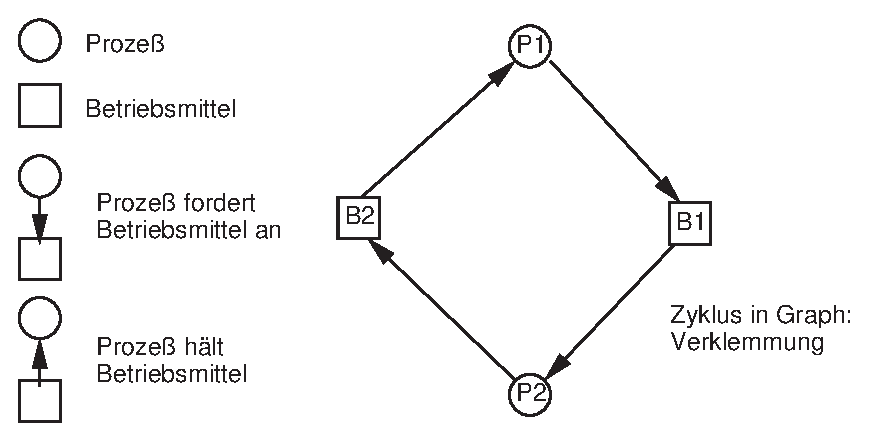
\includegraphics[scale=0.8]{deadlock.eps}%\centerline{\BoxedEPSF{deadlock.epsf  scaled 750}}
	\caption{\label{deadlock} Modellierung einer Verklemmungssituation durch 
	einen Graphen}
\end{figure}

\paragraph{Vier Strategien mit dem Verklemmungsproblem umzugehen:}
\begin{enumerate}
\item   "`Vogel-Strauß"'-Algorithmus (Beispiel: UNIX)
\item   Erkennung und Auflösung (Beispiel: Datenbanktransaktionen)
\item   Verklemmungsfreiheit durch besondere Zuteilungsalgorithmen
	(Verklemmungsvermeidung, \emph{deadlock avoidance})
\item   Verhinderung von Verklemmungen durch Aufheben einer der vier notwendigen
	Bedingungen
\end{enumerate}
\paragraph{Beispiele für Verhinderungsmaßnahmen:}
\begin{enumerate}
\item   mehrfachen Zugriff erlauben (Bedingung 1. ist aufgehoben)\\
	Im allgemeinen nicht sinnvoll.
\item   \emph{preemptive scheduling} (Bedingung 3. ist aufgehoben)\\
	Bei CPU selbstverständlich, bei E/A-Geräten meist nicht sinnvoll.
\item   Vorwegzuteilung aller von einem Prozeß benötigten Betriebsmittel
	\begin{itemize}
	\item   im Prinzip möglich
	\item   Nachteil: Parallelität stark eingeschränkt
	\item   Betriebsmittelbedarf muß im Vorhinein bekannt sein.
	\end{itemize}
\end{enumerate}

\paragraph{Verklemmungsvermeidung} beruht auf der Grundidee, die 
Betriebsmittelanforderungen der Prozesse in eine "`verklemmungsfreie"' 
Reihenfolge zu bringen. Die Algorithmen (Vgl. Bankiersalgorithmus) 
hierfür sind teiweise sehr komplex und auch nur anwendbar, wenn der 
gesamte Betriebsmittelbedarf der Prozesse im vorhinein bekannt ist, was 
in der Praxis häufig nicht der Fall ist. Nichtsdestotrotz hat sich um 
dieses Thema herum eine eigene mathematische Theorie entwickelt, auf die 
hier aber nicht eingegangen wird.

\section{Prozessorverwaltung}
\subsection {Funktion des Schedulers}
\paragraph{Kurzfristige Steuerung (\emph{short term scheduling}):}
Zuteilung von Betriebsmitteln (hier CPU) zu Prozessen, sobald ver"-füg"-bar, bei
möglichst guter Auslastung der Betriebsmittel und fairer Behandlung aller
Prozesse. Sie stellt die Synchronisationsprimitive zur Verfügung.

(Daneben gibt es die - hier nicht behandelte - mittelfristige Steuerung, 
die auf der Job-Ebene angesiedelt ist und einzelnen Prozessen bzw. Jobs 
z.B. auf der Basis von Benutzerklassen oder des zu erwartenden Speicher- 
und Rechenzeitbedarfs Prioritäten für die Betriebsmittelvergabe zuweist.)
 
Für die folgenden Betrachtungen gehen wir von einer Systemkonfiguration 
aus, bei der die Zahl der Prozesse im Hauptspeicher größer ist als die Zahl 
der Prozessoren.
\paragraph{Prozeßbeschreibung}
\subparagraph{Prozeßzustände:}
\begin{itemize}
\item   \textbf{beendet}\\
	Prozeß, der beendet bzw. nicht vorhanden ist.
\item   \textbf{rechnend}\\
	Prozeß, dem ein Prozessor zugeordnet ist.
\item   \textbf{wartend}\\
	Prozeß, der auf den Eintritt eines Ereignisses wartet.
\item   \textbf{bereit}\\
	Prozeß, der gestartet oder fortgesetzt werden kann, dem aber noch kein
	Prozessor zugeteilt wurde.
\end{itemize}
Abbildung \ref{Zustandsübergänge} zeigt die möglichen 
Zustandsübergänge. Im folgenden werden die diese Übergänge 
auslösenden Operationen bzw. Situtationen beschrieben.
\begin{figure}
    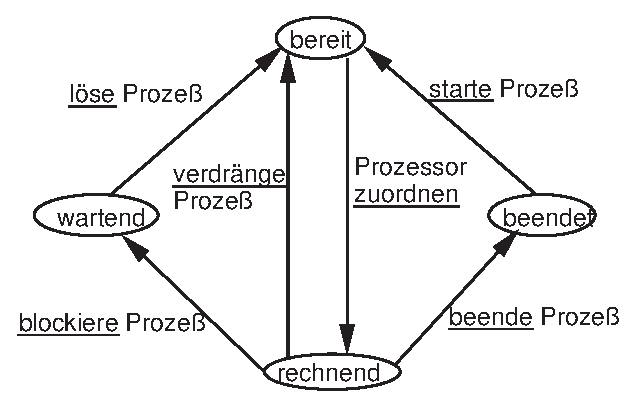
\includegraphics[scale=0.8]{prozessdiagramm.eps}%\centerline{\BoxedEPSF{prozessdiagramm.epsf  scaled 750}}
	\caption{\label{Zustandsübergänge} Mögliche Zustandsübergänge für 
	einen Prozeß}
\end{figure}
Der Übergang vom Zustand \texttt{rechnend} in den Zustand \texttt{bereit} 
erfolgt hier durch die sogenannte \emph{Verdrängung} (\emph{preemptive 
scheduling}) - auch \emph{unterbrechende Steuerung} genannt. Der 
einfachere Fall, daß ein Prozeß den Prozessor von sich aus abgibt 
(Prozeß rechnet bis er fertig ist), wird hier nicht weiter betrachtet.
 
\subparagraph{Prozeßkontrollblöcke:} \ \\
Das Betriebssystem (genauer: der Scheduler) verwaltet die Prozesse in 
einer aus \emph{Prozeßkontrollblöcken} (PKB) bestehenden Prozeßtabelle:.
\ttfamily\\
PKB=registerfeld[1..n]\\
\hspace*{5mm}
\{für die Aufnahme der Registerinhalte incl PC\}\\
prozeßtabelle[1..p] von PKB\\
\hspace*{5mm}
\{Index identifiziert Prozeß\}\\
\rmfamily

Ein Prozeß ist durch seinen PKB und seinen Zustand beschrieben. 
Für die unterbrechende
Steuerung ist ein Zeitgeber erforderlich, der den Prozessor periodisch
unterbricht und den Scheduler aufruft. Die Intervallänge bestimmt den 
Rhythmus der Prozessorzuteilung. Sehr kurze Intervalle bringen viel 
"`Overhead"', sehr lange Intervalle behindern eventuell Prozesse höherer 
Priorität.

\begin{minipage}{6cm}
Zeitgeber:
\ttfamily
\begin{tabbing}
\hspace*{5mm}\=\hspace{5mm}\=\kill
wiederhole\\
\>	Uhr:=intervalllänge\\
\>	wiederhole\\
\>	\>	uhr:=uhr-1\\
\>	bis uhr=0\\
\>	setze interrupt\\
ständig\\
\end{tabbing}
\end{minipage}
\begin{minipage}{6cm}
Befehlszyklus:
\ttfamily
\begin{tabbing}
\hspace*{5mm}\=\hspace{10mm}\=\kill
wiederhole\\
\>	wenn\>	interrupt und intErlaubt\\
\>	dann\>	rücksetze interrupt\\
\>	\>	interruptbehandlung\\
\>	\>	monitor(verdrängeProzeß)\\
\>	führe aktuellen Befehl aus\\
ständig
\end{tabbing}
\end{minipage}

Die \texttt{interruptbehandlung} prüft die Ursache der Unterbrechung und 
führt die Routine 
\texttt{monitor(verdrängeProzeß)} nur dann aus, wenn die Unterbrechung durch
den Zeitgeber ausgelöst wurde. Da alle Prozessoren denselben 
\texttt{monitor} benutzen, stellt dieser einen kritischen Abschnitt dar.
Der \textbf{Monitor} hat folgenden Aufbau:

\bigskip
\begin{minipage}{6cm}
\ttfamily
\begin{tabbing}
\hspace*{5mm}\=\hspace{5mm}\=\kill
monitor(funktion)\\
\>	teste und setze(sm)\\
\>	prozeßtabelle[aktiverProzeß].registerfeld:=Prozessorregister\\
\>	CASE funktion\\
\>	\>	$\left.\begin{array}{l}\vdots\\\mbox{verdrängeProzeß}\\\vdots\end{array}\right\}\mbox{\textrm{scheduling}}$\\
\>	prozeß:=aktiverProzeß\\
\>	Prozessorregister:=prozeßtabelle[prozeß].registerfeld\\
\>	sm:=1\\
end-monitor
\end{tabbing}
\end{minipage}

\bigskip
Das Retten und Zurückholen der Prozessorregister bezeichnet man auch als
\emph{context switching}.
\texttt{aktiverProzeß} ist aus der Menge der rechenwilligen Prozesse zu
ermitteln (verwaltet in einer Liste, der \texttt{bereitliste}).
Die \texttt{bereitliste} kennt zwei Funktionen:
\begin{itemize}
\item	\texttt{einfüge(prozeß,bereitliste)}, um einen Prozeß der Liste
	hinzuzufügen
\item	\texttt{entferne(prozeß,bereitliste)}, um einen Prozeß aus der Liste zu
	entfernen
\end{itemize}

\bigskip
Mithilfe dieser Funktionen kann die Monitorroutine 
\texttt{verdrängeProzeß} implementiert werden.

\bigskip
\begin{minipage}{6cm}
\ttfamily
\begin{tabbing}
\hspace*{5mm}\=\hspace{5mm}\=\kill
verdrängeProzeß\\
\>	einfüge(prozeß,bereitliste)\\
\>	entferne(prozeß,bereitliste)
\end{tabbing}
\end{minipage}

\bigskip
Die Bereitsliste enthält immer mindestens einen rechenwilligen Prozeß, 
den sogenannten Nullprozeß, der bei der Systeminitialisierung zum 
aktiven Prozeß gemacht wird.

\paragraph{Weitere scheduler-Routinen}:

\bigskip
\begin{minipage}{6cm}
\ttfamily
\begin{tabbing}
\hspace*{5mm}\=\hspace{5mm}\=\kill
starteProzeß(anfangszustand)\\
\>	hole freien PKB(neuerProzeß)\\
\>	prozeßtabelle[neuerProzeß].registerfeld:=anfangszustand\\
\>	einfüge(neuerProzeß,bereitliste)
\end{tabbing}
\end{minipage}

\smallskip
\begin{minipage}{6cm}
\ttfamily
\begin{tabbing}
\hspace*{5mm}\=\hspace{5mm}\=\kill
beende(prozeß) \{Prozeß beendet sich selbst\}\\
\>	PKB freigeben\\
\>	entferne(aktiverProzeß,bereitliste)
\end{tabbing}
\end{minipage}

\paragraph{Semaphoroperationen}

Die im Abschnitt 2.2 beschriebenen Semaphoroperationen \texttt{up} und 
\texttt{down} können auch als 
Monitorroutinen implmentiert werden. Dabei ist jeder Semaphore folgende 
Struktur zugeordnet:
\begin{verbatim}
	semaphore[sem] = record
	                   zaehler
	                   warteschlange
	                 end
\end{verbatim}
Damit ergibt sich für \texttt{up} und 
\texttt{down}:
\begin{verbatim}
	down(sem):
	   wenn semaphore[sem].zaehler > 0
	   dann semaphore[sem].zaehler := semaphore[sem].zaehler - 1
	        aktiverProzess := prozess {oder verdraenge(prozess)}
	   sonst einfuege(semaphore[sem].warteschlane, prozess)
	         entferne(bereitliste, aktiverProzess)
	
	up(sem):
	   wenn nicht leer(semaphore[sem].warteschlange)
	   dann entferne(semaphore[sem].warteschlange, aktiverProzess)
	        eifuege(bereitliste, aktiverProzess)
	   sonst semaphore[sem].zaehler := semaphore[sem].zaehler + 1
	   aktiverProzess := prozess {oder verdraenge(prozess)}
\end{verbatim}

Diese Implementierungen benutzen nicht mehr die "`beschäftigte Form des 
Wartens"'.

\subsection{Steuerungsstrategien (\emph{scheduling strategies})}
\begin{enumerate}
\renewcommand{\labelenumi}{\alph{enumi})}
\item	\textbf{\emph{round robin} scheduling:}\\
	Jeder Prozeß erhält ein festes Zeitquantum. Wenn dieses abgelaufen ist,
	wird auf den nächsten Prozeß umgeschaltet. Der unterbrochene Prozeß
	kommt ans Ende der \texttt{bereitliste}. Es handlet sich um eine 
	einfache, faire und häufig benutzte Strategie.\\
	Parameter: Länge des Zeitquantums
	\begin{itemize}
	\item	zu kurz: Verwaltungsaufwand (\emph{context switching}) wird sehr hoch
	\item	zu lang: Antwortzeiten werden lang
	\end{itemize}
	Erfahrungswert: $100ms$
\item	\textbf{Prioritätssteuerung:}\\
	Prozesse haben unterschiedliche Prioritäten und werden danach eingeplant.
	Nur der Prozeß mit der höchsten Priorität darf rechnen. Um 
	"`Langläufer"' zu "`bremsen"' könnte der Scheduler die Priorität
	schrittweise vermindern. Die Priorität kann \emph{statisch}
	oder \emph{dynamisch} zugeordnet werden. Bei dynamischer Zuordnung 
	ändert sich die Priorität nach bestimmten Regeln:
	\begin{itemize}
	\item	I/O-bound $\to$ hohe Priorität
	\item	CPU-bound $\to$ niedrige Priorität
	\end{itemize}
	Einfache Zuordnungsformel: $p=\frac{1}{f}$, mit $f=$ benutzter Anteil
	des Prozesses an der Rechenzeit während des letzten Zeitquantums.
	
	\smallskip
	\textbf{Erweiterung durch Prioritätsklassen:}
	\begin{itemize}
	\item	Jeder Prozeß wird einer Klasse zugeordnet.
	\item	Innerhalb einer Klasse wird nach \emph{round robin} scheduling verfahren
	\end{itemize}
	Prozesse der zweiten Klasse werden erst bedient, wenn die höchste Klasse
	leer ist.
\item	\textbf{\emph{shortest job first}:}\\
	Diese Methode ist anwendbar für Prozesse, deren Gesamtrechenzeit bekannt
	ist (z.B. \emph{batch-jobs}).
	\textbf{Beispiel:}
	angenommene Jobfolge:\\
	\begin{tabular}{lrrrrr}
	Job-Nr.: & 1 & 2 & 3 & 4 & 5 \\
	CPU-Zeit: & 20 & 10 & 50 & 15 & 5
	\end{tabular}\\
	Die durchschnittliche Rechenzeit (Verweildauer) ergibt:\vspace{1ex}\\
	\begin{minipage}{5.5cm}
	in der Reihenfolge:
	\[ \begin{array}{rrl}
	1: & 20 \\
	2: & 30 \\
	3: & 80 \\
	4: & 95 \\
	5: & 100 & \\ \hline
	\sum & 325 & \div 5 = 65
	\end{array} \]
	\end{minipage}
	\begin{minipage}{5.5cm}
	shortest job first:
	\[ \begin{array}{rrl}
	5: & 5 \\
	2: & 15 \\
	4: & 30 \\
	1: & 50 \\
	3: & 100 & \\ \hline
	\sum & 200 & \div 5 = 40
	\end{array} \]
	\end{minipage}\\
	
	\smallskip
	$\Rightarrow$ Die durchschnittliche Rechenzeit wird minimiert.
\item	\textbf{guaranteed scheduling:}\\
	z.B. Realzeitsysteme
%\item	\textbf{Beeinflussung von Prioritäten durch Benutzerprozesse:}\\
%	z.B. Datenbanksysteme
\item	\textbf{Scheduling mit Verdrängung von Prozessen}\\
	\begin{itemize}
	\item	Auslagern eines Prozesses (\emph{swapping})
	\item	zwei-Ebenen-Scheduling\\
		1.Ebene: Scheduling der Prozesse im Hauptspeicher\\
		2.Ebene: Ein-/Auslagern von Prozessen
	\end{itemize}
\end{enumerate}
\section{Zusammenfassung}
Sequentielle Prozesse sind Abstraktionsmittel, um von Details auf
Maschinenebene (z.B. Interrupts) abstrahieren zu können
Ein Betriebssystem ist eine Sammlung parallel ablaufender sequentieller
Prozesse. Jeder Prozeß hat eigene virtuelle Betriebsmittel.

Weitere wichtige Konzepte:
\begin{itemize}
\item	Konzept des kritischen Abschnittes
\item	Prozeß-Synchronisations-Primitive
\item	Prozeßzustände
\item	Scheduling-Strategien
\end{itemize}
